% 01_Introduction
\chapter{Introduction}

TODO: Write some text. Write some Introduction for your application.


%%%%%%%%%%%%%%%%%%%%%%%%%%%%%%%%%%
% 02_Installation
%%%%%%%%%%%%%%%%%%%%%%%%%%%%%%%%%%
\chapter{Installation}
SBMLsimulator comes as a Java JAR file. It can run out-of-the-box on all systems where a Java virtual machine is installed and does not require any further installations.


\section{Requirements}
\subsection{Software}

SBMLsimulator is entirely written in Java\TTra and runs on any operating system
where a suitable Java Virtual Machine (JDK version 1.6 or newer) is installed.
See, for example, the Java SE download
page\footnote{\url{http://www.oracle.com/technetwork/java/javase/downloads/index.html}\label{fn:jvmldl}}.

\subsection{Hardware}

With at least 1\,GB main memory, you should be able to perform most tasks
without any problem. An active internet connection is not required for simulations, but for some other application features (e.g., online update).

\section{Starting the application}
\label{startingTheProgram}

If you downloaded a ZIP-file, you need to unzip it before starting the
application. Depending on your operating system, you should use the provided
shell scripts for starting the application. This is \texttt{start.sh} for Linux
or \texttt{start.bat} for Windows. On MAC OS, you have to create your own
shortcut. You can start the application on all operating systems by typing

\begin{lstlisting}[language=bash,numbers=none]
java -jar -Xms128m -Xmx1024m SBMLsimulator.jar
\end{lstlisting}

\noindent on your command prompt. Please note that you might have to change
\texttt{SBMLsimulator.jar} for the real name of the JAR-file, e.g.,
\texttt{SBMLsimulator-1.0-rc2-full.jar}. In this example, a minimum of 128\,MB and a maximum
of 1024\,MB of memory will be available for the program. In most cases,
SBMLsimulator needs more than 128\,MB memory, so it might be convenient to create a
shortcut and start the application with as much memory as available. If you
have 2\,GB RAM, for example, you might want to start the application with the
following command:

\begin{lstlisting}[language=bash,numbers=none]
java -Xms128m -Xmx1400M -jar SBMLsimulator.jar
\end{lstlisting}

For your convenience, we already created several start-scripts to run the
application with as much memory as possible. How much memory you actually need
strongly depends on the size of your input datasets.
%


\chapter{How to get started}

TODO: Write "You need an sbml model and experimental data to perform simulations", etc. text

\section{Prepare experimental data}
\label{ch:prepare}

First of all, make sure that your experimental data is in one of the required file formats. The application can read character separated value (CSV) files, which are mostly tab-separated tabular files with microarray data. To use EXCEL-data, you can simply open your EXCEL spreadsheet, click "File" and "Save as" and select "Tab-separated text file".
For all files, we require one column called "Time" that should contain the timepoints as rowindex. We further required multiple other columns, which you may want to call s1, s2,\dots or c1,c2,\dots TODO: ICH HAB KEINE AHNNUNG WAS DAS IST! BITTE BESCHREIBEN

\subsection{Experimental data example}
As described, you need a rowindex column with the timepoints and multiple columns that state the concentration of each metabolite at each timepoint (TODO: IST DAS KORREKT?). The following is an example how an input file may look like:

Example:
\begin{lstlisting}[caption={Input file example for experimental data},label={lst:input:exp},numbers=none,captionpos=t,float=h]
Time    s1          s2          s3
0       32.456E-12  7.02        12E32
4       5E-54       179.05E-14  0.005
...     ...         ...         ...
\end{lstlisting}

\section{Open experimental data in the application}
\label{sec:opendata}

\begin{figure}[h]
\centerline{\noindent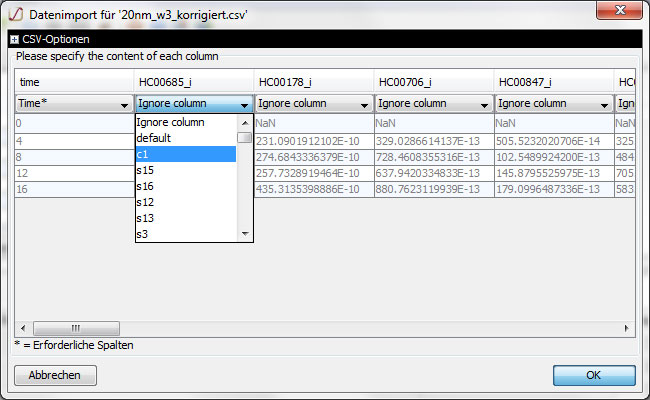
\includegraphics[width=1.0\columnwidth]{figures/import_dialog.jpg}}
\caption{
Example of the data import dialog. The "CSV Options" panel might be expanded to correct auto-detected input file properties. At the table in the lower half, the content of each column must be specified.
}\label{fig:inputdialog}
\end{figure}

In general, all data must be processed expression data in tabular text files (see Section~\ref{ch:prepare} for descriptions and examples of the input file formats). Then, there are many possibilities to open datasets in SBMLsimulator. For example, you can simply drag\&drop data into the application or select "File", "Open" to open a file. 

Figure~\ref{fig:inputdialog} shows an example of the file input dialog. If the input file format has not been inferred automatically, one may click on the black "CSV Options" label to specify further options (like "column separator char" or if the file contains headers - see Figure~\ref{fig:csvoptions}).


\begin{figure}[h]
\centerline{\noindent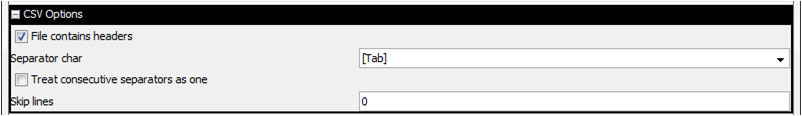
\includegraphics[width=1.0\columnwidth]{figures/expanded_csv_options.jpg}}
\caption{
Expanded "CSV Options" allow to give details for the input file. These properties are auto-detected and only need to be changed if the auto-detection failed to correctly infer those properties.
}\label{fig:csvoptions}
\end{figure}

In the table at the lower half of this dialog, one must specify the content of each column. This can be done by clicking on the combo box below the captions. 

\chapter{Command-line arguments and preferences}

TODO: Export the options with command-line name, GUI name and tooltip as LaTeX.

% 03_Troubleshooting
\chapter{FAQ / Troubleshooting}
\label{ch:faq}

TODO: These are some template questions. Add new ones and modify/ remove the
old ones to suit your needs.

\noindent \textbf{Where can I get help for a certain component/ option/ checkbox/ etc.?}\newline
Most elements in SBMLsimulator have tooltips. If you don't understand an option, you
can get help in the first place by just pointing the mouse cursor over it and
wait for the tooltip to show up ($\sim$ 3 seconds).\newline

\noindent \textbf{I'm getting a ``java.lang.OutOfMemoryError: Java heap space"}\newline
Some operations need a lot of memory. If you simply start SBMLsimulator, without any
JVM parameters, only 64\,MB of memory are available. Please append the argument
\texttt{-Xmx1024M} to start the application with 1\,GB of main memory. See
Section~\vref{startingTheProgram} for a more detailed description of how to
start the application with additional memory. If possible, you should give the
application 2\,GB of main memory. A minimum of 1\,GB main memory should be
available to the application.\newline

\noindent \textbf{Is an internet connection required to run SBMLsimulator?}\newline
An internet connection is not required for simulations, but for some other operations, like the online-update feature.\newline

\noindent \textbf{Where can I get the latest version?}\newline
Go to \url{http://www.cogsys.cs.uni-tuebingen.de/software/SBMLsimulator/}.\newline

\noindent \textbf{Which Java version must be installed on my computer to launch
SBMLsimulator?}\newline SBMLsimulator requires at least Java 1.6. Please see
\url{http://www.java.com/de/download/} to download the latest Java version.

\noindent \textbf{Why does SBMLsimulator not start on my Mac with Mac OS prior to
10.6 Update 3?}\newline If you try to launch SBMLsimulator, but the application does
not start and you receive the following error message on the command-line or
Java console of your Mac, you need to update your Java installation:
\begin{verbatim}
Exception in thread "AWT-EventQueue-0" java.lang.NoClassDefFoundError:
    com/apple/eawt/AboutHandler
    at java.lang.ClassLoader.defineClass1(Native Method)
    at java.lang.ClassLoader.defineClass(ClassLoader.java:703)
    ...
\end{verbatim}
The interface \texttt{com.apple.eawt.AboutHandler} was introduced to Java for
Mac OS X 10.6 Update 3. If you have an earlier version of Mac OS or Java,
please update your OS or Java installation. Also see the Mac OS documentation
about the \texttt{AboutHandler} for more information. On a Mac, you can update
your Java installation through the Software Update menu item in the main Apple
menu.

